Resultados: Deberán analizar y comparar las implementaciones de las funciones en su versión de la cátedra en C y la suya en assembler y mostrar los resultados obtenidos a través de tablas y gráficos. Para esto deberán plantear experimentos que les permitan medir el rendimiento y comparar entre las implementaciones. Deberán además explicar detalladamente los resultados obtenidos y analizarlos. En el caso de encontrar anomalías o comportamientos no esperados deberán construir nuevos experimentos para entender qué es lo que sucede.

\subsection{Eficiencia c vs paralelismo simd asm}
- función solver set bnd:
se evaluó el código en assembler, llamado asm, y código c de la función solver set bound sobre seis tamaños distintos de matrices. al variar parámetro b, valores de 1,2,3 y 10, se obtienen promedios similares en caso de matriz con tamaño 512x512 (ver tabla), sacando outliers. los resultados se mantienen alrededor de 18500 ticks para asm y 54000 ticks para c. 
repetimos escenario con matriz de tamaño 16x16, variando b en mismos valores que para tamaño 512x512. aunque se nota 
variación de tiempos entre mediciones no se nota gran cambio en los resultados, manteniendose el promedio de tiempos c alrededor de 2000 ticks y tiempos asm alrededor de 350 ticks.
a causa de esto y de que no queremos llenar de gráficas innecesarias hemos decidido fijar el parámetro b en 2 para restantes experimentaciones de función. 
se muestra en figura gráfica de ejecución de los códigos, donde para cada tamaño se ejecutaron 100 veces.
\begin{figure}[h]

\centering
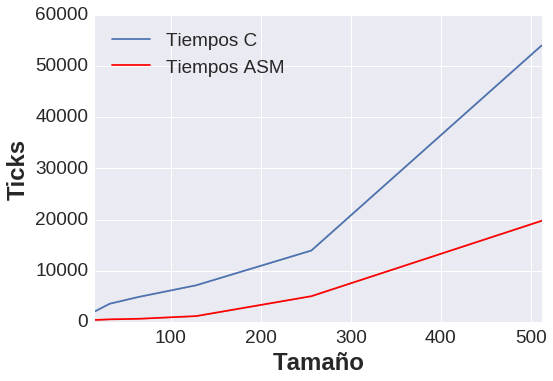
\includegraphics[scale=0.6] {grafC}
  
 \caption{Tiempos en ticks de ejecución de código C vs código ASM}
\end{figure}



